\documentclass[tikz]{standalone}
\usepackage{physics}
\usetikzlibrary{decorations.markings,arrows.meta}

\begin{document}
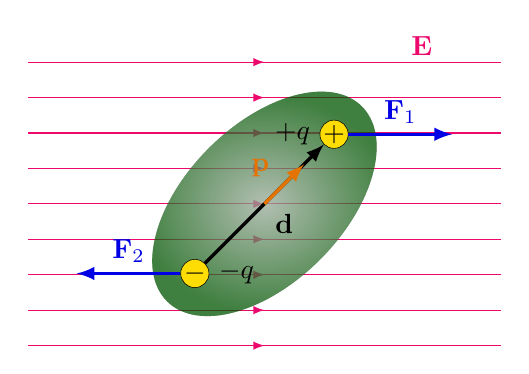
\begin{tikzpicture}[decoration={markings,
        mark= at position 0.5 with {\arrow{latex}}}
  ]
  % E-field
  \def\n{8}
  \def\l{1.8}
  \foreach \i in{0,...,\n}{
      \draw[thin,postaction={decorate},magenta!70!red] (-3,-2*\l/\n*\i+\l) -- (3,-2*\l/\n*\i+\l);
    }
  \node[magenta!70!red] at (2,2){$\vb{E}$};

  % Ellipse
  \fill[outer color=green!50!black,inner color=green!10,rotate=45,opacity=0.5] (0,0) ellipse (1.75 and 1);

  % Charges
  \node[circle,draw, very thin,fill=yellow!80!orange,inner sep=0] (pos) at (0.884,0.884){$+$};
  \node[anchor=east] at (pos.west){$+q$};
  \node[circle,draw, very thin,fill=yellow!80!orange,inner sep=0] (neg) at (-0.884,-0.884){$-$};
  \node[anchor=west] at (neg.east){$-q$};

  % Vectors
  \draw[very thick,-latex] (neg.north east) -- node[anchor=north west]{$\vb{d}$} (pos.south west);
  \draw[very thick,-latex,blue!90!black] (pos.east) -- node[anchor=south]{$\vb{F}_1$} (2.384,0.884);
  \draw[very thick,-latex,blue!90!black] (neg.west) -- node[anchor=south]{$\vb{F}_2$} (-2.384,-0.884);
  \draw[very thick,-latex,blue!90!black,orange!90!black] (0,0) -- node[anchor=south east,pos=0.4]{$\vb{p}$} (0.5,0.5);


  % Angle

\end{tikzpicture}
\end{document}